\documentclass[
	%parspace, % Térköz bekezdések közé / Add vertical space between paragraphs
	%noindent, % Bekezdésének első sora ne legyen behúzva / No indentation of first lines in each paragraph
	%nohyp, % Szavak sorvégi elválasztásának tiltása / No hyphenation of words
	%twoside, % Kétoldalas nyomtatás / Double sided format
	%draft, % Gyorsabb fordítás ábrák rajzolása nélkül / Quicker draft compilation without rendering images
	%final, % Teendők elrejtése / Set final to hide todos
]{elteikthesis}[2020/11/23]

% Dolgozat metaadatai
% Document's metadata
\title{Tervezési minták a Játékfejlesztésben} % cím / title
\date{2021} % védés éve / year of defense

% Szerző metaadatai
% Author's metadata
\author{Hajdu Marcell Ferenc}
\degree{programtervező informatikus BSc}

% Témavezető(k) metaadatai
% Superivsor(s)' metadata
\supervisor{Kovácsné Pusztai Kinga Emese} % belső témavezető neve / internal supervisor's name
\affiliation{egyetemi tanársegéd} % belső témavezető beosztása / internal supervisor's affiliation
%\extsupervisor{Külső Kornél} % külső témavezető neve / external supervisor's name
%\extaffiliation{informatikai igazgató} % külső témavezető beosztása / external supervisor's affiliation

% Egyetem metaadatai
% University's metadata
\university{Eötvös Loránd Tudományegyetem} % egyetem neve / university's name
\faculty{Informatikai Kar} % kar neve / faculty's name
\department{Algoritmusok és Alkalmazásai\\ Tanszék} % tanszék neve / department's name
\city{Budapest} % város / city
\logo{elte_cimer_szines} % logo

% Irodalomjegyzék hozzáadása
% Add bibliography file
\addbibresource{thesis.bib}

% A dolgozat
% The document
\begin{document}

% Nyelv kiválasztása
% Set document language
\documentlang{magyar}
%\documentlang{english}

% Teendők listája (final dokumentumban nincs)
% List of todos (not in the final document)
%\listoftodos[\todolabel]

% Dokumentum beállítások
% Some document settings
% Lábjegyzet folytonos számozása fejezetek között
% Continuous counting of footnotes among chapters
\counterwithout{footnote}{chapter}

% Tartalomjegyzék oldalszámozásának rejtése
% Hide page numbering of ToC
\newcounter{conpageno}
\let\oldtableofcontents\tableofcontents
\renewcommand{\tableofcontents}{
	\pagenumbering{gobble}
	\oldtableofcontents
	\cleardoublepage
	\setcounter{conpageno}{\value{page}}
	\pagenumbering{arabic}
	\setcounter{page}{\value{conpageno}}
}


% Címlap (kötelező)
% Title page (mandatory)
\maketitle
\topicdeclaration

% Tartalomjegyzék (kötelező)
% Table of contents (mandatory)
\tableofcontents
\cleardoublepage

% Tartalom
% Main content
\chapter{Bevezetés} % Introduction
\label{ch:intro}

\cleardoublepage

\chapter{Felhasználói dokumentáció} % User guide
\label{ch:user}

\section{A játék rövid leírása}
A játék Hack-and-Slash stílusú. A célunk, hogy haladjunk előre egy pályán, ahol különböző nehézségű és számosságú ellenfelek jönnek velünk szembe. A pályán találhatunk felvehető tárgyakat, amik szituációtól függően erősítenek bennünket. Halál esetén újraéledünk egy előre meghatározott ellenőrző ponton, ahonnan folytathatjuk a játékot. A pálya végén értékel minket a játék, és ha más játékosokhoz képest (mint egy árkád játékban, local high score) jobban teljesítettünk, vagy még nem telt be az eredménytábla, akkor az előbb említett táblára felkerülünk. A játék 3 pályát/szintet tartalmaz, amik egyre nehezebbek, ezen felül állásunkat el tudjuk mentei, valamint betölteni. Mindezzel egy kohézív gyors, kihívásokkal teli játékélményt kínálunk.
\subsection{Célközönség}
A játék azon eberek számára lehet érdekes, akik szeretik a gyors kihívással teli árkát stílusú Hack-and-Slash játékokat. 15 életévet minimum betöltött embernek ajánljuk, mivel a játék vért és erőszakot (ellenfelek legyőzése) tartalmaz.
\cleardoublepage
\section{Rendszerkövetelmények}
\begin{table}[htb]
	\centering
	\begin{tabular}{ | m{0.1\textwidth} | m{0.4\textwidth} | m{0.4\textwidth} | }
		\hline
		\textbf{Adatok} & \textbf{Minimum követelménye} & \textbf{Ajánlott követelmény} \\
		\hline \hline
		CPU & Intel i5-8250U & Intel i5-8600K \\ \hline
		GPU & Nvidia GeForce MX150 & Nvidia GTX 1050Ti \\ \hline
		RAM & 8Gb & 16Gb \\ \hline
		OS & \multicolumn{2}{c|}{Windows, Linux} \\
		\hline
		Disc & \multicolumn{2}{c|}{300Mb} \\
		\hline
	\end{tabular}
	\caption{rendszerkövetelmények}
	\label{sysReq}
\end{table}
\subsection{Játék indítása}
A játék nem igényel telepítést. Futtatásához indítsa el a 'The Quest for the Thesis.exe'-t (kattintson rá bal egérgombbal kétszer Windows-on).

\cleardoublepage
\section{Funkciók ismertetése}
A következő fejezetekben a játék funkcióinak részletesebb ismertetése lesz kifejtve. Hogyan is néz ki a játék, és mivel találkozhatunk miután elindítottuk.

\subsection{Grafikus Felhasználói Interfész (GUI)}
Kettőféle Grafikus Felhasználói Interfész különböztethetünk meg a játék során. Az egyik, ami tisztán információt közöl velünk, a másik amivel interaktálhatunk is.
\subsubsection{Tisztán információ közlő GUI-k}
Játékon belüli indikátorok azok a grafikus elemek, amik visszajelzik nekünk a játékos aktuális állapotát. 
\begin{figure}[htb]
	\noindent\makebox[\textwidth]{
	\includegraphics[width= 1\textwidth]{inUse}}
	\caption{Játékon belüli indikátorok}
	\label{inUse}
\end{figure}

Itt látható a játékos jelenlegi élete.
\begin{figure}[htb]
	\noindent\makebox[\textwidth]{
	\includegraphics[width= 1\textwidth]{inUseHealth}}
	\caption{Játékos életereje}
	\label{inUseHealth}
\end{figure}

A játékos képességei és tárgyai, valamint az idő addig amíg újra lehet használni a tárgyat/képességet.
\begin{figure}[htb]
	\noindent\makebox[\textwidth]{
	\includegraphics[width= 1\textwidth]{inUseItems}}
	\caption{Játékos képességei és tárgyai}
	\label{inUseItems}
\end{figure}

Valamint a játékost éppen érintő státuszeffekteket.
\begin{figure}[htb]
	\noindent\makebox[\textwidth]{
	\includegraphics[width= 1\textwidth]{inUseStatuses}}
	\caption{Játékost érintő státuszeffekteket}
	\label{inUseStatuses}
\end{figure}

Ezeken felül ebbe a kategóriába tartozik még a töltőképernyő, ami a szintek között jelenhet meg.
\begin{figure}[H]
	\noindent\makebox[\textwidth]{
	\includegraphics[width= 1\textwidth]{loading}}
	\caption{Töltőképernyő}
	\label{loading}
\end{figure}

\cleardoublepage
Valamint a halálképernyő, ami akkor jelenik meg, ha a játékos meghalt.
\begin{figure}[H]
	\noindent\makebox[\textwidth]{
	\includegraphics[width= 1\textwidth]{dead}}
	\caption{Halálképernyő}
	\label{dead}
\end{figure}

\subsubsection{Interaktív GUI-k}
Ezeken a képernyőkön vannak gombok, lenyíló listák, vagy csúszkák, amikkel interaktálhatunk a játékkal.

\begin{enumerate}
	\item \label{fomenu} \textbf{Főmenü} az első GUI elem amit látunk a játék indításakor. Öt gomb látható ezen a felületen:
	\begin{itemize}
		\item \textit{Start} ha erre a gombra kattintunk akkor tovább lépünk a \textit{Pályaválasztóra \ref{levelSelector}}.
		\item \textit{Settings} erre kattintva megnyitjuk a \textit{Beállítások \ref{setting}} menüt.
		\item \textit{Score Board}-ra kattintva eljutunk az \textit{Eredménytáblára \ref{scoreboard}}.
		\item \textit{Credit} gombra kattintva eljutunk a \textit{Köszönetnyilvánító \ref{credit}} menüre.
		\item \textit{Exit} gomb lenyomásával kilépünk a játékból.
	\end{itemize}
	\begin{figure}[H]
		\noindent\makebox[\textwidth]{
		\includegraphics[width= 1\textwidth]{mainMenu}}
		\caption{A Kezdőképernyő}
		\label{mainMenu}
	\end{figure}
	
	\item \label{levelSelector} \textbf{Pályaválasztó} menün  adhatjuk meg a nevünket ami később az \textit{Eredménytáblán \ref{scoreboard}} látható.
	\begin{itemize}
	\item A \textit{Easy, Medium} és \textit{Hard} gombok lenyomásával átléphetünk az \textit{Utasítások \ref{instructions}} menübe, és a játék betölti a megfelelő pályát.
	\item \textit{Load} gomb lenyomását követően átlépünk a \textit{Mentés és Betöltés \ref{save}} menübe.
	\end{itemize}
	\begin{figure}[H]
		\noindent\makebox[\textwidth]{
		\includegraphics[width= 1\textwidth]{levelSelection}}
		\caption{A Pályaválasztó menü}
		\label{levelSelection}
	\end{figure}
	
	\item \label{instructions} \textbf{Utasítások} menüben láthatók a játék bemeneteire végrehajtott akciók.
	\begin{itemize}
		\item \textit{Play} gomb lenyomását követően elkezdődik a játék.
	\end{itemize}
	\begin{figure}[H]
		\noindent\makebox[\textwidth]{
		\includegraphics[width= 1\textwidth]{instructions}}
		\caption{Utasítások menü}
		\label{instructionsF}
	\end{figure}	
	
	\item \label{scoreboard} \textbf{Eredménytábla} ahol a szinteken elért eredmények láthatók.
	\begin{itemize}
		\item \textit{Back} gomb lenyomását követően visszatérünk az előző menübe.
	\end{itemize}
	\begin{figure}[H]
		\noindent\makebox[\textwidth]{
		\includegraphics[width= 1\textwidth]{scoreBoard}}
		\caption{Eredménytábla}
		\label{scoreBoardF}
	\end{figure}
	
	\item \label{credit} \textbf{Köszönetnyilvánító} menün található a játék készítéséhez felhasznált assetek készítői.
	\begin{itemize}
		\item \textit{Back} gomb lenyomását követően visszatérünk az előző menübe.
	\end{itemize}
	\begin{figure}[H]
		\noindent\makebox[\textwidth]{
		\includegraphics[width= 1\textwidth]{credit}}
		\caption{Köszönetnyilvánító menü}
		\label{creditF}
	\end{figure}
	
	\item \label{setting} \textbf{Beállítások} menüben változtathatjuk meg az alapértelmezett beállításainkat.
	\begin{itemize}
		\item Bal felül választhatjuk ki egy lenyíló listából a kívánt felbontást.
		\item Jobb felül választhatjuk ki egy lenyíló listából a játékablak üzemmódját.
		\item \textit{Graphics Quality} menüpontban egy lenyíló listából kiválaszthatjuk a játék minőségi beállításait.
		\item \textit{Main Volume} csúszkán a fő hangerőt tudjuk állítani.
		\item \textit{Music Volume} csúszkán a zene hangerejét tudjuk állítani.
		\item \textit{SFX Volume} csúszkán az effektek hangerejét tudjuk állítani.
		\item \textit{Back} gomb lenyomását követően visszatérünk az előző menübe.
	\end{itemize}
	\begin{figure}[H]
		\noindent\makebox[\textwidth]{
		\includegraphics[width= 1\textwidth]{settings}}
		\caption{Beállítások}
		\label{settings}
	\end{figure}
	
	\item \label{save} \textbf{Mentés és Betöltés} menün található a 4 mentési hely. Ahol ha már volt mentésünk akkor a mentésben szereplő adatok jelennek meg, ha nem akkor az \textit{Empty Slot} felirat.   
	\begin{itemize}
		\item \textit{Load} gombot megnyomva a kijelölt mentés fog betölteni.
		\item \textit{Save} gombra kattintva a kijelölt mentési helyre elmentődik a jelenlegi állás (csak játék közben látható).
		\item \textit{Back} gomb lenyomását követően visszatérünk az előző menübe.
	\end{itemize}
	\begin{figure}[H]
		\noindent\makebox[\textwidth]{
		\includegraphics[width= 1\textwidth]{saveLoad}}
		\caption{Mentés és Betöltés menü}
		\label{saveLoad}
	\end{figure}
	
	\item \label{pause} \textbf{Szünet} menüt a játék közben az \textbf{ESC} gomb lenyomásával hívhatjuk elő.
	\begin{itemize}
		\item \textit{Resume} gomb lenyomását követően a játék folytatódik.
		\item \textit{Save / Load} gombot megnyomva továbblépünk a \textit{Mentés és Betöltés \ref{save}} menüre.
		\item \textit{Exit} gomb lenyomását követően a játék bezáródik.
	\end{itemize}
	\begin{figure}[H]
		\noindent\makebox[\textwidth]{
		\includegraphics[width= 1\textwidth]{pause}}
		\caption{Szünet menü}
		\label{pauseF}
	\end{figure}
	
	\item \label{end} \textbf{Vég} menü egy pálya végén jelenik meg.
	\begin{itemize}
		\item Legfelül látható a pálya elvégzését követő eredményünk.
		\item A szerzett pontunk alatt láthatóak a többi pályákat reprezentáló gombok, amik re kattintva a megfelelő pálya betöltődik (különböző pályákról érkezve a Vég menübe más pályák jelennek meg itt).
		\item \textit{Load} gombot megnyomva továbblépünk a \textit{Mentés és Betöltés \ref{save}} menüre.
		\item \textit{Score Board}-ra kattintva eljutunk az \textit{Eredménytáblára \ref{scoreboard}}.
		\item \textit{Credit} gombra kattintva eljutunk a \textit{Köszönetnyilvánító \ref{credit}} menüre.
		\item \textit{Exit} gomb lenyomását követően a játék bezáródik.
	\end{itemize}
	\begin{figure}[H]
		\noindent\makebox[\textwidth]{
		\includegraphics[width= 1\textwidth]{end}}
		\caption{Vég menü}
		\label{endF}
	\end{figure}
	
\end{enumerate}

\subsection{Pályák}
A játékban három pályát különítünk el: Easy, Medium, Hard

\begin{itemize}
	\item \textbf{Easy} pálya a névből eredően a legkönnyebb. A tárgyak és az ellenfelek megismerésére tökéletesen alkalmas.
	\begin{figure}[H]
		\noindent\makebox[\textwidth]{
		\includegraphics[width= 1\textwidth]{easy}}
		\caption{Easy pálya}
	\end{figure}
		\cleardoublepage
		\item \textbf{Medium} pálya közepes nehézségű. Több ellenség érkezik felén és a felvehető tárgyak ritkák.
	\begin{figure}[H]
		\noindent\makebox[\textwidth]{
		\includegraphics[width= 1\textwidth]{medium}}
		\caption{Medium pálya}
	\end{figure}
	
		\item \textbf{Hard} pálya a legnehezebb. A tárgyak kevesek, az ellenségek számosak és az erősebb fajtából valók.
	\begin{figure}[H]
		\noindent\makebox[\textwidth]{
		\includegraphics[width= 1\textwidth]{hard}}
		\caption{Hard pálya}
	\end{figure}
\end{itemize}

\subsection{Irányítás}
\begin{table}[H]
	\centering
	\begin{tabular}{ | m{0.3\textwidth} | m{0.5\textwidth} | }
		\hline
		\textbf{Akció} & \textbf{Gomb} \\
		\hline \hline
		Bal irányú mozgás & A \\ \hline
		Jobb irányú mozgás & D \\ \hline
		Ugrás & SPACE \\ \hline
		Gyors hirtelen mozgás & Baloldali ALT \\ \hline
		Sima Támadás & Baloldali egérgomb \\ \hline
		1, 2, 3, 4 gombok & megfelelő helyen lévő tárgy használata \\ \hline
		Tárgyak felvétele & E \\ \hline
		Játék megállítása & ESC \\ \hline
	\end{tabular}
	\label{instruc}
\end{table}

\subsection{Tárgyak}
\begin{table}[H]
	\centering
	\begin{tabular}{ | m{0.2\textwidth} | m{0.2\textwidth} | m{0.4\textwidth} | N |}
		\hline
		\textbf{Név} & \textbf{Kép} & \textbf{Leírás} & \\
		\hline \hline
		Gyógyító ital & 
			\noindent\makebox[0.2\textwidth]{
			\includegraphics[width= 0.2\textwidth]{CurePotion}}
		& Megszünteti az összes státuszeffektust.
		& \label{que:curePotion}
		\\ \hline
		
		Életerő ital & 
			\noindent\makebox[0.2\textwidth]{
			\includegraphics[width= 0.2\textwidth]{HealthPotion}}
		& Gyógyítja a játékost és a \textit{Gyógyul \ref{que:healing}} státuszeffektet rakja rá.
		& \label{que:healthPotion}
		\\ \hline		
		
		Tűz varázsfókusz & 
			\noindent\makebox[0.2\textwidth]{
			\includegraphics[width= 0.2\textwidth]{FireMagicFocus}}
		& Lehetővé teszi a \textit{Tűzkarika \ref{que:fireBurst}} varázslat használatára a játékost.
		& \label{que:fireMagicFocus}
		\\ \hline
		
		Jég varázsfókusz & 
			\noindent\makebox[0.2\textwidth]{
			\includegraphics[width= 0.2\textwidth]{IceMagicFocus}}
		& Lehetővé teszi a \textit{Jéglándzsa \ref{que:iceLance}} varázslat használatára a játékost.
		& \label{que:iceMagicFocus}
		\\ \hline
		
		Katana & 
			\noindent\makebox[0.2\textwidth]{
			\includegraphics[width= 0.2\textwidth]{Katana}}
		& Egy egyszerű kard amivel sebzed az ellenségeket.
		& \label{que:katana}
		\\ \hline
		
		Masamune & 
			\noindent\makebox[0.2\textwidth]{
			\includegraphics[width= 0.2\textwidth]{Masamune}}
		& Gyengén sebzi az ellenségeket, azonban \textit{Vérzés \ref{que:bleeding}} státuszeffektet rak rájuk.
		& \label{que:masamune}
		\\ \hline
		
		Muramasa & 
			\noindent\makebox[0.2\textwidth]{
			\includegraphics[width= 0.2\textwidth]{Muramasa}}
		& Erősen megsebzi az ellenségeket, és \textit{Kábult \ref{que::stunned}} státuszeffektet rak rájuk, azonban alacsony a támadási sebessége.
		& \label{que:muramasa}
		\\ \hline
		
	\end{tabular}
\end{table}

\subsection{Varázslatok}
\begin{table}[H]
	\centering
	\begin{tabular}{| m{0.2\textwidth} | m{0.2\textwidth} | m{0.4\textwidth} | N |}
		\hline
		\textbf{Név} & \textbf{Kép} & \textbf{Leírás} & \\
		\hline \hline
		
		Tűzkarika & 
			\noindent\makebox[0.2\textwidth]{
			\includegraphics[width= 0.2\textwidth]{fireBurst}}
		& Rengeteg sebzést okoz az összes közeli ellenségnek, és az \textit{Égés \ref{que:burning}} státuszeffektet rakja rájuk, nagy az újrahasználási ideje.
		& \label{que:fireBurst}
		\\ \hline
		
		Jéglándzsa & 
			\noindent\makebox[0.2\textwidth]{
			\includegraphics[width= 0.2\textwidth]{iceLance}}
		& Megsebzi az ellenségeket, és \textit{Fagyás \ref{que:frozen}} státuszeffektet rak rájuk.
		& \label{que:iceLance}
		\\ \hline
		
	\end{tabular}
\end{table}

\subsection{Státuszeffektusok}

\begin{table}[H]
	\centering
	\begin{tabular}{| m{0.2\textwidth} | m{0.2\textwidth} | m{0.4\textwidth} | N |}
		\hline
		 \textbf{Név} & \textbf{Kép} & \textbf{Leírás} &\\
		\hline \hline
		
		Vérzés & 
			\noindent\makebox[0.15\textwidth]{
			\includegraphics[width= 0.15\textwidth]{Bleeding}}
		& Időközönként megsebzi kicsit a célpontot.
		& \label{que:bleeding}
		\\ \hline
		
		Égés & 
			\noindent\makebox[0.15\textwidth]{
			\includegraphics[width= 0.15\textwidth]{Burning}}
		& Időközönként megsebzi a célpontot.
		& \label{que:burning}
		\\ \hline
		
		Fagyás & 
			\noindent\makebox[0.15\textwidth]{
			\includegraphics[width= 0.15\textwidth]{Frozen}}
		& Időközönként megsebzi és lelassítja a célpontot.
		& \label{que:frozen}
		\\ \hline
		
		Kábult & 
			\noindent\makebox[0.15\textwidth]{
			\includegraphics[width= 0.15\textwidth]{Stunned}}
		& Rendkívül megsebzi a célpontot és lezárja a mozgási lehetőségeit egy időre.
		& \label{que::stunned}
		\\ \hline
		
		Gyógyul & 
			\noindent\makebox[0.15\textwidth]{
			\includegraphics[width= 0.15\textwidth]{Healing}}
		& Időközönként gyógyítja a célpontot.
		& \label{que:healing}
		\\ \hline		
		
	\end{tabular}
\end{table}

\cleardoublepage

\subsection{Ellenfelek}
Minden ellenségnek kettő típusa van: járőr és őr. Az őr egy helybe áll és vár a játékosra. A járőr kettő pont között mozog.
\begin{center}
	\begin{longtable}{| m{0.2\textwidth} | m{0.2\textwidth} | m{0.4\textwidth} | N |}
	%\centering
		\hline
		\textbf{Név} & \textbf{Kép} & \textbf{Leírás} & \\
		\hline \hline
		
		Alap Ellenség & 
			\noindent\makebox[0.2\textwidth]{
			\includegraphics[width= 0.2\textwidth]{enemy}}
		& A leggyengébb ellenség, ami egy \textit{Katanaát \ref{que:katana}} használ a fő fegyvereként.
		& \label{que:enemy}
		\\ \hline
		
		Erős Ellenség & 
			\noindent\makebox[0.2\textwidth]{
			\includegraphics[width= 0.2\textwidth]{strongEnemy}}
		& Egy lényegesen erősebb ellenség, ami egy \textit{Masamunet \ref{que:masamune}} használ a fő fegyvereként.
		& \label{que:strongEnemy}
		\\ \hline		
		
		Tűzvarázsló & 
			\noindent\makebox[0.2\textwidth]{
			\includegraphics[width= 0.2\textwidth]{fireMage}}
		& Egy varázsló egység, ami egy \textit{Muramasat \ref{que:muramasa}} használ a fő fegyvereként, azonban képes a \textit{Tűzgyűrű \ref{que:muramasa}} varázslat használatára is.
		& \label{que:fireMage}
		\\ \hline
		
		Jégvarázsló & 
			\noindent\makebox[0.2\textwidth]{
			\includegraphics[width= 0.2\textwidth]{iceMage}}
		& Egy rendkívül veszélyes varázsló egység, ami egy \textit{Masamunet \ref{que:masamune}} használ a fő fegyvereként és képes a \textit{Jéglándzsa \ref{que:muramasa}} varázslat használatára is.
		& \label{que:iceeMage}
		\\ \hline		
		
	\end{longtable}
\end{center}
\cleardoublepage

\chapter{Fejlesztői dokumentáció} % Developer guide
\label{ch:impl}

\section{Tervezés}

\subsection{Kezdeti tervek}
Mivel egy játék (legyen akármekkora is) egy bonyolult rendszer, és mivel alapértelmezetten is egy jó gyakorlat, a projekt elejétől kezdve meg szerettem volna tervezni, átfogóalga a különböző rendszereket. Tudtam előre, hogy a Unity játékmotort fogom használni a példajáték elkészítéséhez, és a tervminták alkalmazására és fontosságára Jason Weimann\cite{jason}, DapperDino\cite{dapperDino} és a Game Programming Patterns-ben\cite{gameProgrammingPatterns} olvasottak inspiráltak. Azt is figyelmemben tartottam, hogy szakdolgozatom célja a tervezési minták és programozási elvek felhasználása a játékfejlesztésben és nem feltétlenül egy teljes mértékben kidolgozott játék piacra dobása.\\*
Mindezek után három dolgot tartottam fontosnak eleinte, a játékos (és ellenségek) statemachine-ját, egy általánost leírás az alap rendszerek kapcsolatáról, valamint a játékom elkészítése a S.O.L.I.D elvek szerint.
\begin{figure}[H]
	\noindent\makebox[\textwidth]{
	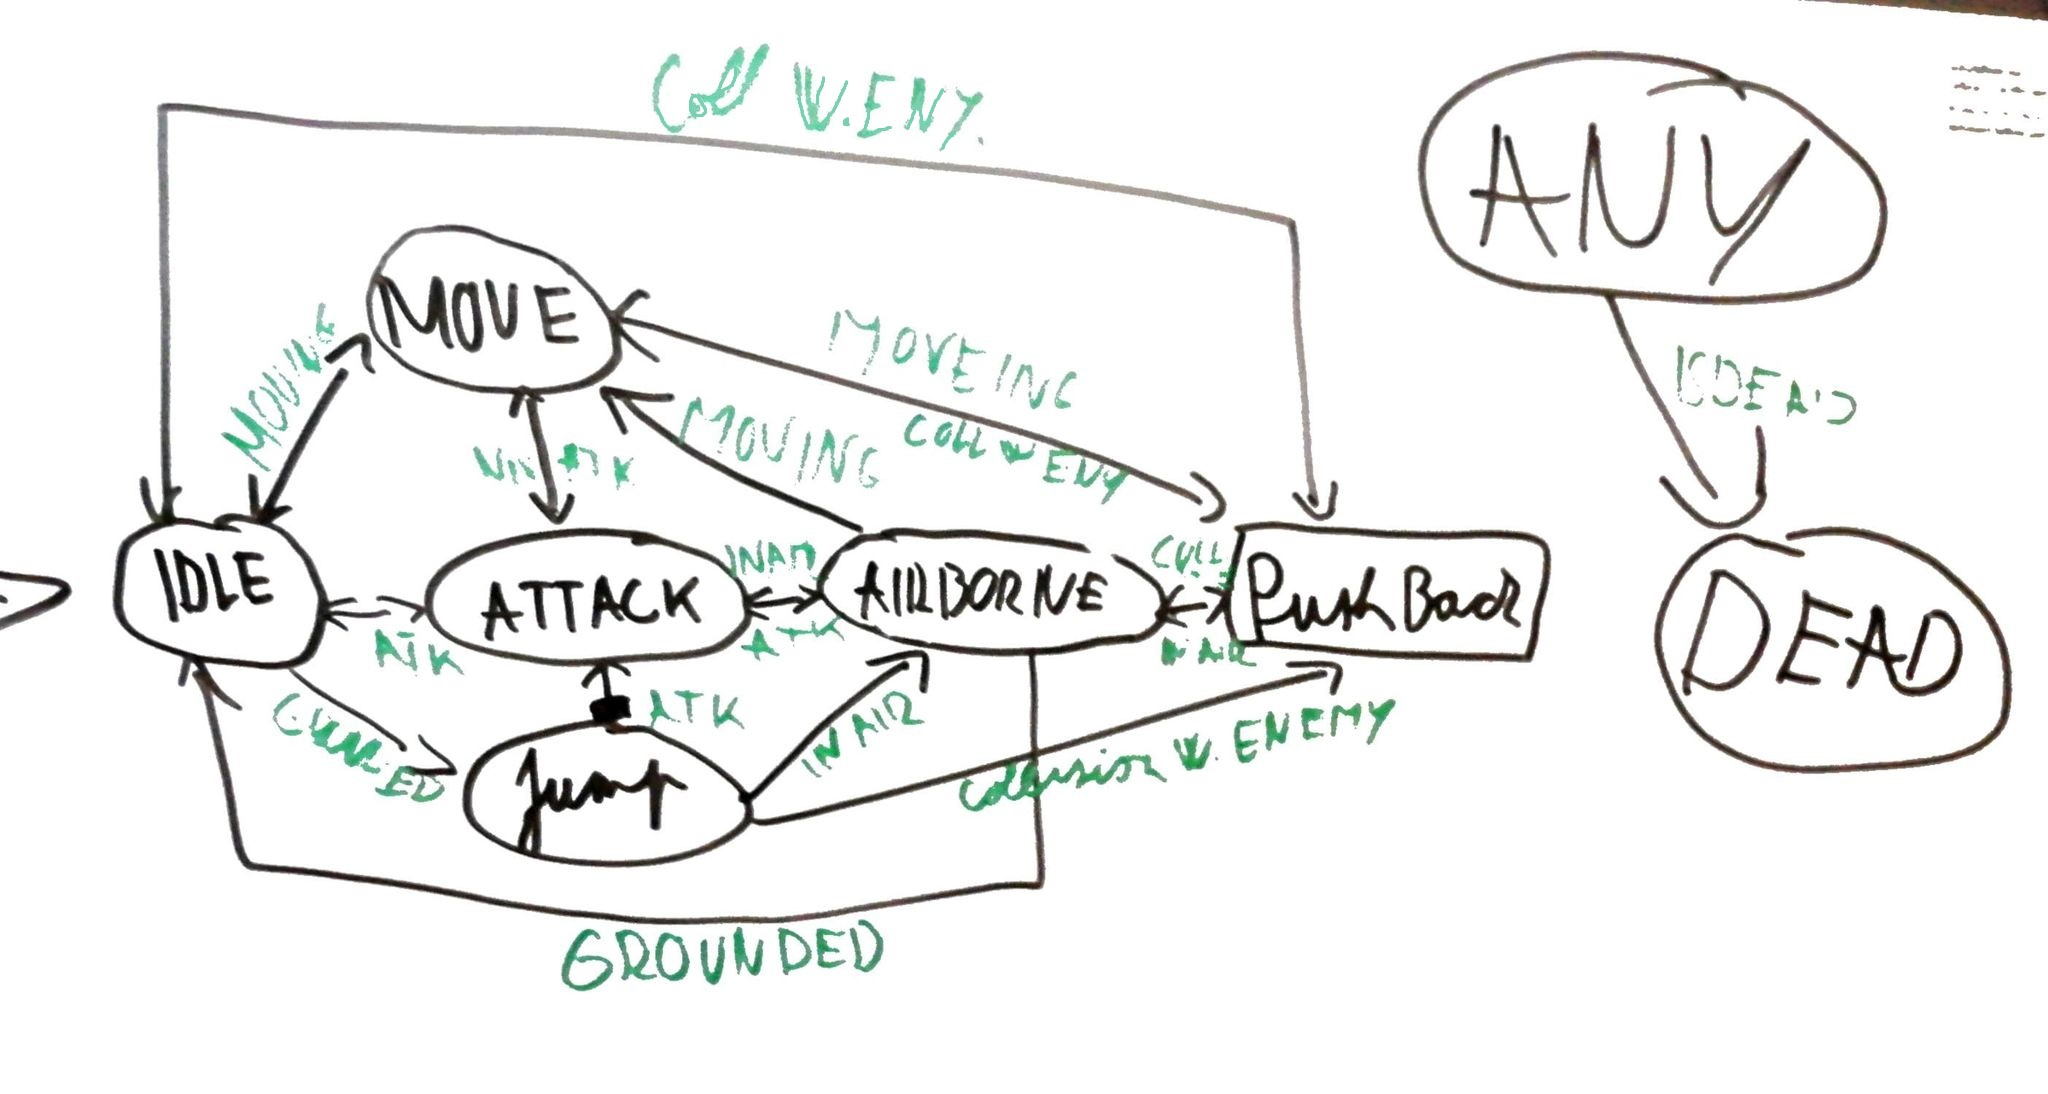
\includegraphics[width= 0.8\textwidth]{statemachine}}
	\caption{Kezdeti statemachine}
	\label{statemachine}
\end{figure}

\begin{figure}[H]
	\noindent\makebox[\textwidth]{
	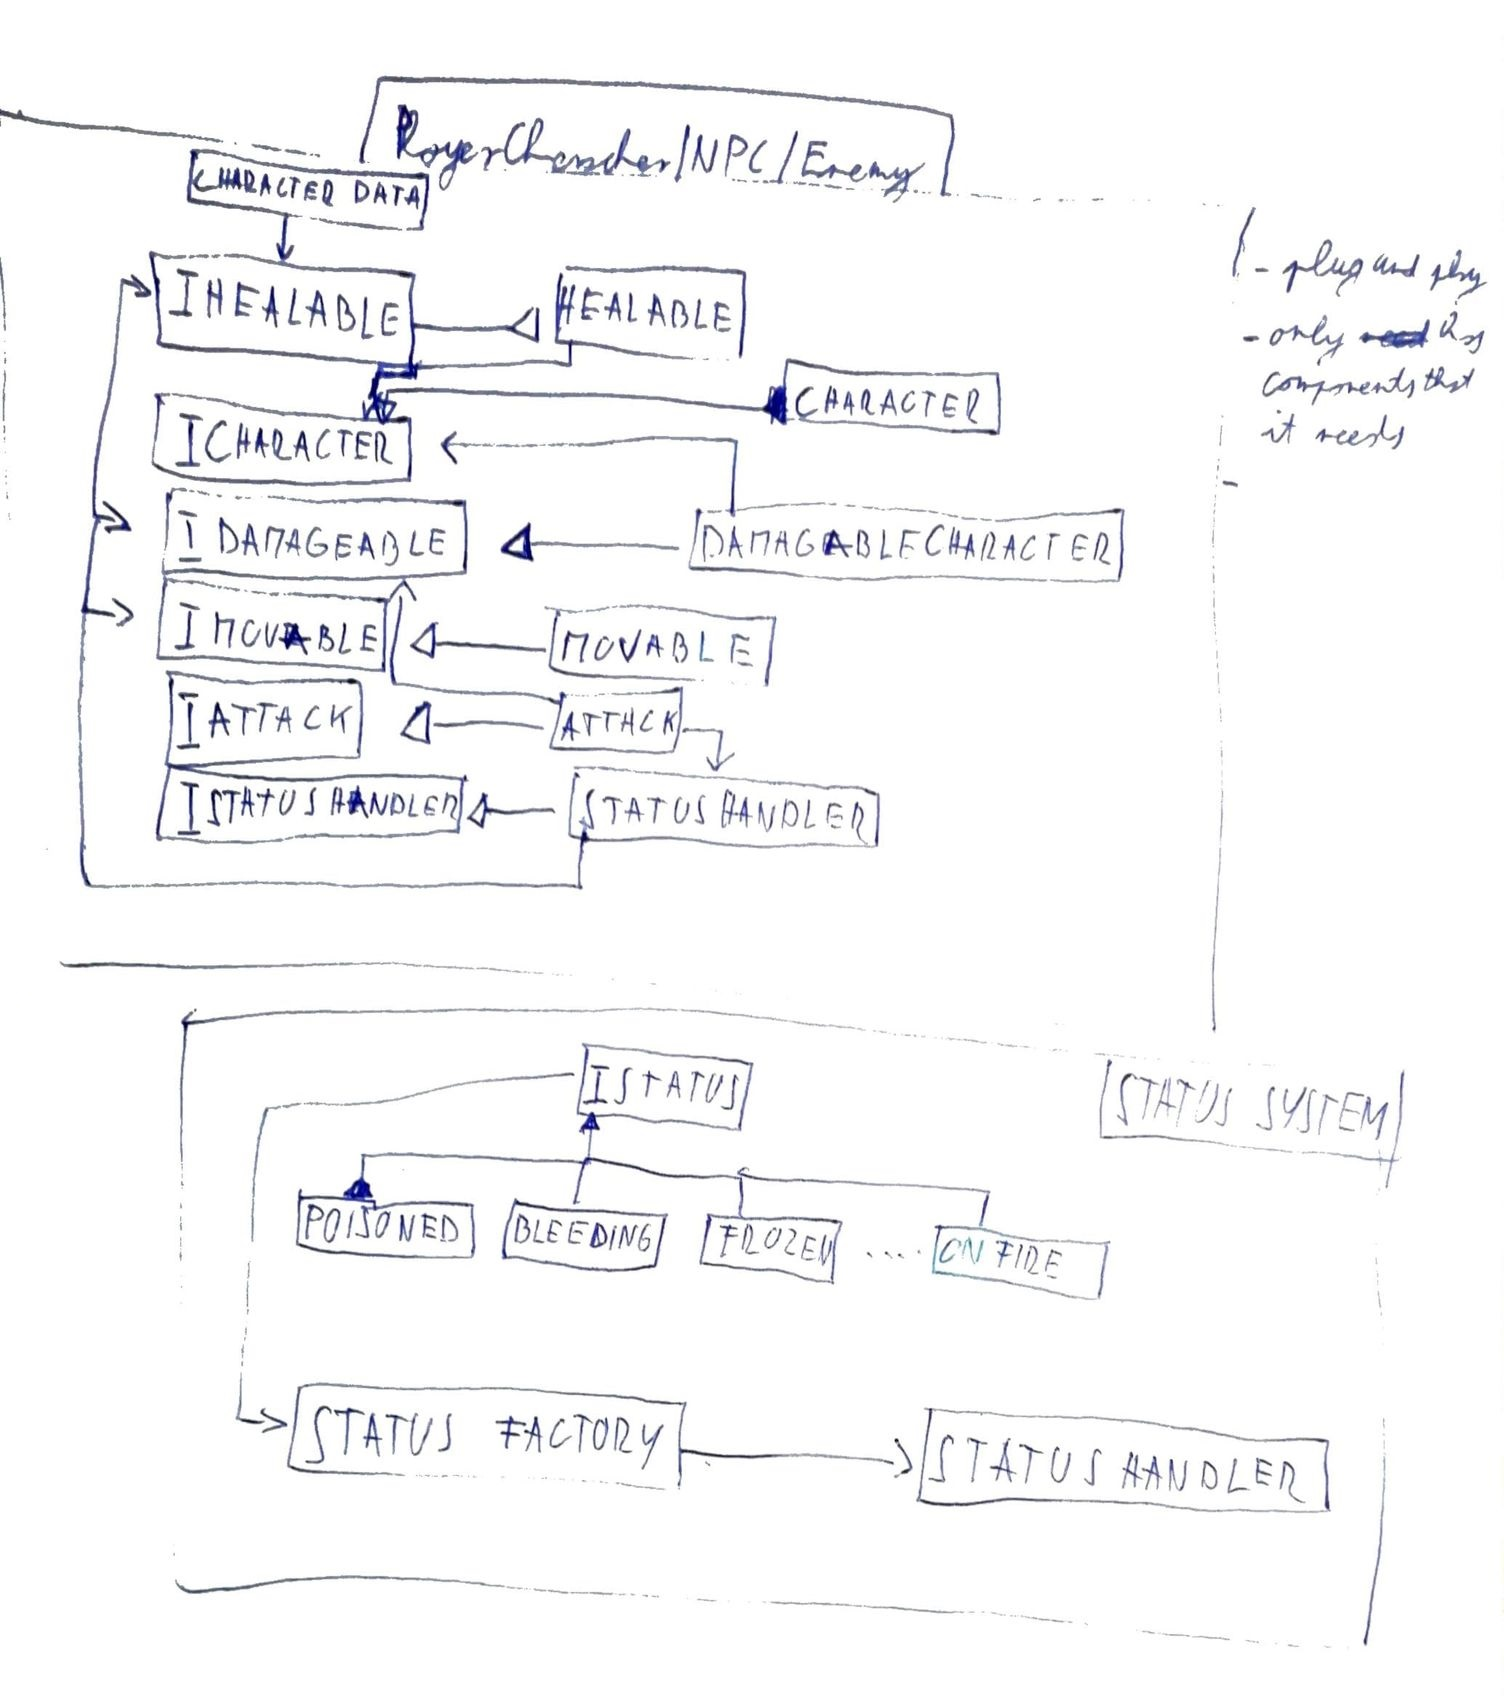
\includegraphics[width= 0.8\textwidth]{statussys}}
	\caption{Rendszerek általános leírása}
	\label{statussys}
\end{figure}

Azonban hamar rájöttem, hogy bizonyos bonyolultan rendszerek kapcsolatát érdemes jobban kifejteni. Ilyen volt a támadással foglalkozó csoport is, ahol három kisebb rendszer összeépítését kellett kivitelezni. Ezek a varázslatok, státuszeffektusok és maga a támadás rendszere voltak.

\begin{figure}[H]
	\noindent\makebox[\textwidth]{
	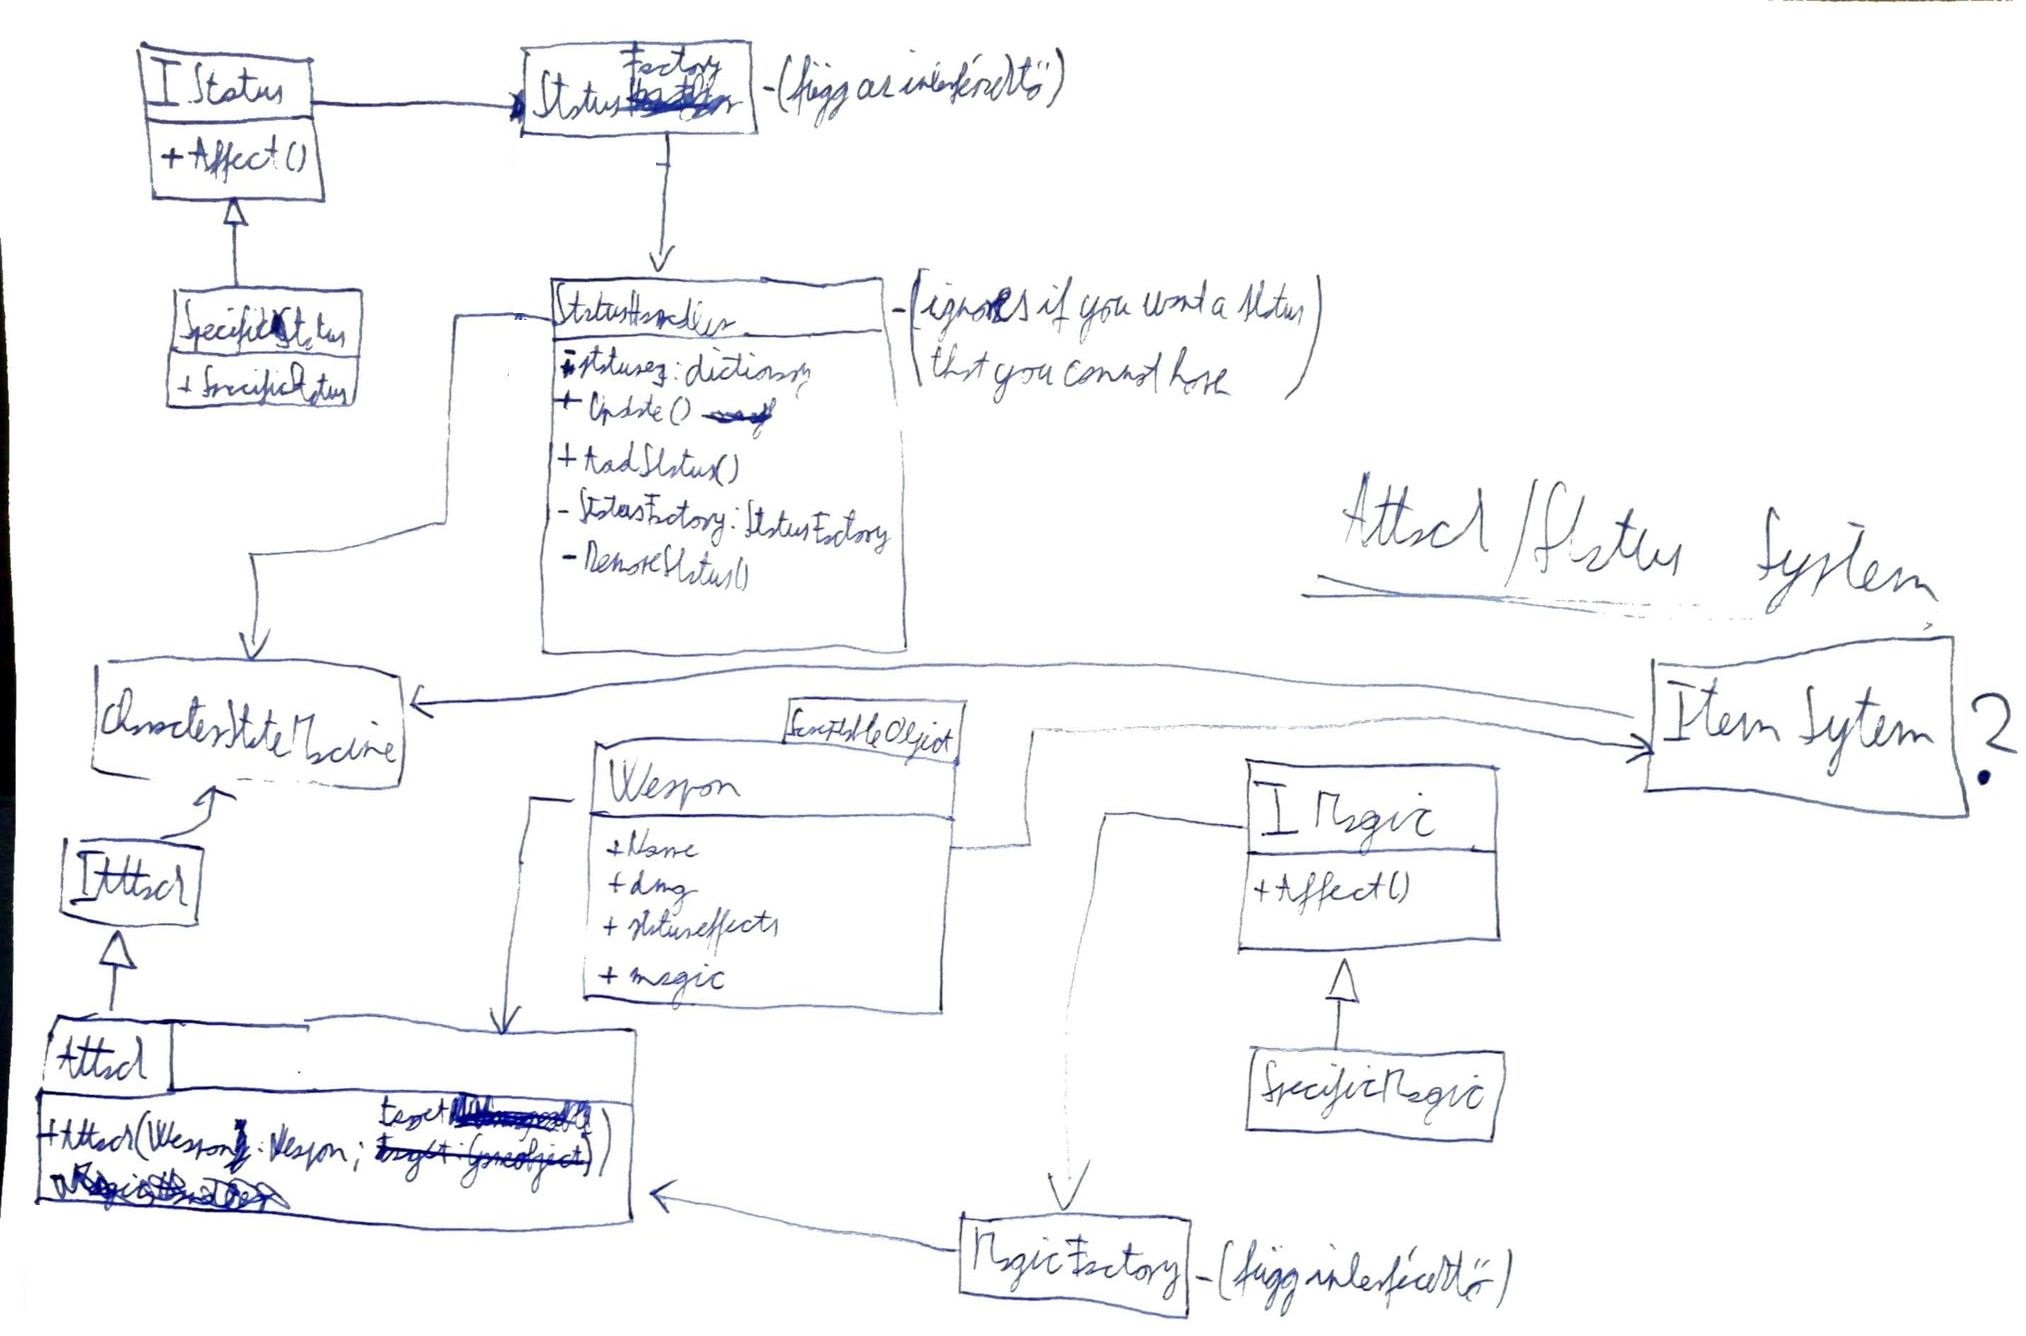
\includegraphics[width= 1\textwidth]{all}}
	\caption{Támadási rendszer}
	\label{all}
\end{figure}

\subsection{Unity}
A Unity játékmotor egy cross-platform komponens alapú játékfejlesztői motor. Ebben a fejlesztői környezetben, relatívan egyszerűen hozhatunk létre játékokat (főleg az új visual scripting segítségével, hiszen így fejlesztők nem kényszerülnek rá a C\# nyelv elsajátítására). Unity-ben 2 fontos dolgot kell megértenünk, egyik az Editor, amit használni fogunk a színterünk komponálására, valamit a komponenseink (GameObjects) létrehozására, a másik a monoBehaviour-ök megértés, hiszen ez az osztály az összes Unity script ősosztálya.\\
Először is a \textbf{Unity Editor}-ról beszélnék. Ez a Unity Engine gafikus interfésze, innen érhetjük el a Unity által biztosított funkciókat, mint például az \textit{animator}, ahol animációk átmeneteit határozhatjuk meg, a \textit{shader graph}-ot, ahol egy grafikus felületen készíthetünk vertex és fragment shader-eket, vagy akár a \textit{test runner}-t, hogy párat említsek.\\*
Azonban a 2 legfontosabb funkciója az Editornak a színtereink(scenes) és \textit{gameObject}-jeink komponálása. A színtereinken készíthetünk pályákat, menüket, adhatunk hozzá hangforrásokat, fényeget vagy utóhatások, nem mellesleg ide kell hozzáadnuk a gameObject-eket, hogy megjelenjenek.\\*
A \textit{gameObject}-ekteket el lehet képzelni úgy, mint egy üres dobozt,amihez különböző komponenseket adhatunk. Ha azt akarjuk, hogy ne láthatatlan legyen a dobozunk adhatunk hozzá egy \textit{Sprite Renderer}-t, ha akarjuk, hogy a fizika hasson rá akkor hozzáadhatjuk a \textit{Rigidbody} komponenst és így tovább. Egy gameObject rengeteg minden lehet és több funkciót is elláthat, nem mellesleg rájuk aggathatjuk a saját script-jeinket is hogy valami egyedi hatást/viselkedést érjünk el.\\
Most hogy beszéltem az Editor-ról, a helyről, ahol a játék építése folyik beszélnék egy kicsit az egyik legfontosabb építőelemről, a \textbf{monoBehaviour}-ről, ami az összes script-ünk ősosztálya, amit egy \textit{gameObject}-re rá akarunk rakni, mint egy komponenst. A monoBehaviour és minden leszármazottja egy olyan osztály, amit nem lehet a \textbf{new} kulcsszóval példányosítani, csak az \textit{addComponent} függvénnyel. Ebből következve ezen osztályok, csak egy \textit{gameObject}-en élhetnek és kötöttek annak élettartalmához.\\*
A monoBehaviour biztosít számunkra pár fontos metódust is \cite{unityDocs}.
\begin{itemize}
	\item \textbf{Start} - inicializációs fázis utolsó lépése.
	\item \textbf{FixedUpdate} - fizikai frissítés. Itt lehet olyan fizikai számításokat kezelni, amiket minden ütemezett fizikai frissítésben végre akarunk hajtani.
	\item \textbf{OnCollisionXXX} - mi történjen ha valami ütközés történik.
	\item \textbf{Update} - elépzelhető mint egy monoBehaviour-re korlátozott \textit{gameLoop}. Akkor használjuk, ha ismétlődő számításokat akarunk végrehajtani (minden frame-ben).
\end{itemize}

\begin{figure}[H]
	\noindent\makebox[\textwidth]{
	\includegraphics[width= 1\textwidth]{thdfT}}
	\caption{MonoBehaviour életciklusa}
	\label{thdfT}
\end{figure}

\subsection{S.O.L.I.D.}
A S.O.L.I.D. elvek\cite{solid}

\textbf{S - Single-responsiblity Principle}, avagy az \textit{Egyetlen felelősség elve}\\
Ennek az elvnek a lényege, hogy egy osztálynak, egyetlen egy oka lehet a változásra, vagyis egy céljának kell lennie. Ennek az elvnek a megvalósítása Unity-ben triviális, hiszen kisebb odafigyeléssel ez adódik is a komponens alapú összetételből.

\textbf{O - Open-closed Principle}, avagy az \textit{Nyílt/zárt elv}\\
Itt a legfontosabb tudnivaló, hogy egy objektumnak képesnek (nyitottnak) kell lennie a bővítésekre, azonban ezeknek a bővítéseknek nem szabad módosítania a meglévő osztályt, zárva kell lennie a módosításokra tekintve. Ugye ez az elv interfészek és ősosztályok megvalósításával könnyen elérhető, hiszen ha megvannak a mintáink, hogy miképp kell egy osztálynak felépülnie, és azt meg is valósítottuk, esetleg egységtesztekkel le is védtük működését, akkor annak módosítása hiba nélkül nehéz lesz, azonban a bővítése triviális. Az a fontos itt, hogy a régi kódban lévő logika a bővítés miatt ne kényszerüljön az új kódrész függésére, ebben az esetben lehet érdemes meggondolni a kód faledarabolását a \textit{Egyetlen felelősség elve} mintájára.

\textbf{L - Liskov Substitution Principle}, avagy az \textit{Liskov helyettesítési elv}\\
Liskov helyettesítési elv lényege, hogy minden osztályt be kéne tudni helyettesíteni annak ősosztályába, interfészébe. Ez egy rendkívül fontos megállapítás, hiszen ezzel meg tudjuk szüntetni a függést egy specifikus osztályimplementációtól, ezáltal képesek leszünk könnyen cserélni konkrét működést egy komponensben/osztályban annak megváltoztatása nélkül.

\textbf{I - Interface Segregation Principle}, avagy az \textit{Interfész elválasztási elv}\\
Az elv azt mondja ki, hogy egy osztálynak nem szabad függenie olyan interfészektől, függvényektől, amiket nem valósít meg, nem használ. Ez könnyen felfogható, úgy mint az \textit{Egyetlen felelősség elve} alkalmazása interfészekre, hiszen így több kisebb közelebb kapcsolódó interfészt kapunk, amiket szabadon implementálhat egy osztály szükség szerűen, ellentétben egy nagy interfésszel.

\textbf{D - Dependency Inversion Principle}, avagy az \textit{Függőség megfordítási elv}\\
Ez az elv azt mondja ki, hogy az entitásoknak absztrakciókon kell függeniük, valamint, hogy magasabb rendű rendszereknek nem szabad függeniük az alacsonyrendűektől. Ezt a komponens alapú Unity-ben könnyen elérhetjük, hiszen ha osztályain egy interfészt implementálnak, ami megfelel az absztrakciónak és ezen osztályainkat a \textit{Liskov helyettesítési elv} és a \textit{Egyetlen felelősség elve} szerint hoztuk létre és mint Unity-s komponens használunk, akkor a magas szintű rendszereink tudnak csak az absztrakciótól függeni és Unity-ben intuitívan megvalósulni.

Mindezeket látva a Unity mint keretrendszer rendkívül alkalmas a S.O.L.I.D. elvek alkalmazására.

\subsection{Tervminták}
Miután átnéztük, hogy milyen elvek szerint lett elkészítve a játék, térjünk is át a szakdolgozat lényegére, a felhasznált tervmintákra és azok hasznára szerepére. A Game Programming Patterns-ben\cite{gameProgrammingPatterns} olvasott tervmintákat, néhány más hasznos mintával kiegészítve fogom kifejteni itt részletesebben, Jason Weimann\cite{jason} és DapperDino\cite{dapperDino} implementációit és példáit alapul véve. Ezek a minták kettő csoportba sorolhatók alapvetően, amik az \textbf{általunk implementált} tervezési minták és a \textbf{Unity/C\# által biztosított} tervezési minták, kezdjük is az utóbbikkal.

\textbf{Game Loop} - avagy a \textit{Játékciklus}\\
Ez a játék magja, legfontosabb alapköve. A Unity automatikusan biztosítja, nincs szükség egy komponáló osztályra, ahol egy while ciklusban hívódnának osztályaink. A tervminta lényeg, hogy biztosítanunk kell egy a játék terminállásáig tartó folyamatos környezetet, ahol a játékos inputot, eseményeket és a játékon belüli időt kezelünk kell. Mivel ezt a modern játékfejlesztői környezetek alapértelmezetten tudják és elrejtik a felhasználó elöl (,mint a Unity), ezért érdemes úgy tekinteni az ezen eszközökkel történő fejlesztés közben, mintha mindig a Játékciklusban lennénk.

\textbf{Update Method} - avagy a \textit{Frissítési metódus}\\
Ez a minta mögött az a gondolat húzódik, hogy vannak bizonyos számítások (például egy karakter pozícióváltozásából származó újrarajzolás) amiket minden egyes kirajzolt frame-ben végre szeretnénk hajtani. Unity-ben ezt a tervmintát még jobban felaprították, hiszen a monoBehaviour biztosít számunkra három különböző Update metódust is. A monoBehaviour életciklusa szerint \textit{FixedUpdate} amiben a fizikai számítások hajtódnak végre fix intervallumonként, \textit{Update}, ami egy általános frissítési metódus, itt végezzük a saját logikánk módosításainak nagyját, legvégül a \textit{LateUpdate}, ami egy a sima Update metódust, animáció frisítéseket és a coroutine-okat követő frissítés, ahol olyan operációkat hajthatunk végre, amiket az Update után szeretnénk végrehajtani.

\textbf{Component} - avagy a \textit{Komponens}\\
Ez a tervminta egy csoportosítási problémát szándékozz megoldani hasonlóan a Egyetlen felelősség elvéhez. Ezt a Unity szintén alapjaiban támogatja, hiszen az egész játékmotor komponens alapú (rigidbody, amiator, spriteRenderer, mint külön komponensek amiket egy gameObject-re tudunk ráaggatni, mint a saját script-jeinket).

\textbf{Type Object/Flyweight} - avagy a \textit{Típusobjektum/Pehelysúlyú}\\
Ezen tervezési minták, habár különböző, azonban egymáshoz rendkívüli módon kapcsolódó koncepciókat írnak le. A Típusobjektum lényeg, hogy a példányspecifikus adatokat a típusolt objektumban tároljuk, míg az ezeket alkalmazó metódusokat/függvényeket, vagy közös adatokat a típusobjektumban definiáljuk, így a közös részeket és az egyedi adatokat elszeparáljuk. A Pehelysúlyú tervminta nagyon hasonlóan el akarja különíteni a példányspecifikus adatokat a megosztott minden azonos osztály számára szükséges és azonos adatoktól, ezáltal létrehozva egy pehelykönnyű osztályt. Mint láthattuk mindkettő tervminta célja a példányspecifikus adatok szeparálása, Unity-ben erre rendkívül jól használhatóak a \textit{ScriptableObject}-ek. Ezek egy különleges osztályok, amik többnyire adatstruktúrákat és közös működéseket írnak le. Miután definiáltunk egy ScriptableObject-et, azt legtöbbször nem a tradícionális módon kódból példányosítjuk, hanem a Unity Editor-ban hozzuk létre, mint új Asset-et, itt tudjuk az általunk megadott mezők értékeit kitölteni. Ha egy a ScriptableObject-et hozzárendelünk GameObject-ekhez akkor a különböző GameObject-ek között a ScriptableObject azonos marad, csak egyszer töltődik be a memóriába és minden változást az összes GameObject lát ha az adott ScriptableObject hozzá van rendelve.

\textbf{Observer} - avagy a \textit{Figyelő}\\
Ez a tervminta annyira elterjedt, hogy a C\# nyelvbe natívan támogatva is van az eseményrendszeren keresztül. Unity-ben is támogatva van a C\#-os eseményrendszer, azonban a Unity-biztosít egy saját eseménykezelést is ez nem más mint a \textit{Unity event}-ek. Ezek lényegében egy kényelmi funkciót látnak el, hogy égszerűen tudjunk az Editor-ban összekötni eseményeket, ezen események általában olyan elemek, amit kóddal ritkán váltunk ki (általában UI gombnyomások vagy az Input System-ből érkező események), azonban saját funkciót szeretnénk kötni különösebb komplikáció nélkül.


\cleardoublepage
\section{Megvalósítás}

\subsection{Felhasználói esetek}
\begin{figure}[H]
	\noindent\makebox[\textwidth]{
	\includegraphics[width= 1.1\textwidth]{useCase}}
	\caption{Felhasználói eset diagram}
	\label{useCase}
\end{figure}

\subsection{Státusz rendszer}

\subsection{Varázslás rendszer}

\subsection{Játékos rendszer}

\subsection{Ellenség rendszer}

\subsection{Adattárolás}

\subsection{GUI}

\subsection{Zene}

\subsection{Pályák felépítése}

\subsection{CI/CD pipeline}


\section{Tesztelés}

\subsection{Egységtesztek}

\begin{figure}[H]
	\noindent\makebox[\textwidth]{
	\includegraphics[width= 1\textwidth]{tests}}
	\caption{Az egységtesztek eredményei}
	\label{tests}
\end{figure}

\begin{figure}[H]
	\noindent\makebox[\textwidth]{
	\includegraphics[width= 1\textwidth]{codeCoverage}}
	\caption{A Logic assembly tesztelési lefedettsége}
	\label{codeCoverage}
\end{figure}


\subsection{Kézi Tesztelés}

\subsection{Tesztelési konklúzió}
\cleardoublepage

\chapter{Összegzés} % Conclusion
\label{ch:sum}


\section{Köszönetnyilvánítás}


\cleardoublepage

% Függelékek (opcionális) - hosszabb részletező táblázatok, sok és/vagy nagy kép esetén hasznos
% Appendices (optional) - useful for detailed information in long tables, many and/or large figures, etc.
\appendix
\chapter{Szimulációs eredmények} % Simulation results
\label{appx:simulation}

Lorem ipsum dolor sit amet, consectetur adipiscing elit. Pellentesque facilisis in nibh auctor molestie. Donec porta tortor mauris. Cras in lacus in purus ultricies blandit. Proin dolor erat, pulvinar posuere orci ac, eleifend ultrices libero. Donec elementum et elit a ullamcorper. Nunc tincidunt, lorem et consectetur tincidunt, ante sapien scelerisque neque, eu bibendum felis augue non est. Maecenas nibh arcu, ultrices et libero id, egestas tempus mauris. Etiam iaculis dui nec augue venenatis, fermentum posuere justo congue. Nullam sit amet porttitor sem, at porttitor augue. Proin bibendum justo at ornare efficitur. Donec tempor turpis ligula, vitae viverra felis finibus eu. Curabitur sed libero ac urna condimentum gravida. Donec tincidunt neque sit amet neque luctus auctor vel eget tortor. Integer dignissim, urna ut lobortis volutpat, justo nunc convallis diam, sit amet vulputate erat eros eu velit. Mauris porttitor dictum ante, commodo facilisis ex suscipit sed.

Sed egestas dapibus nisl, vitae fringilla justo. Donec eget condimentum lectus, molestie mattis nunc. Nulla ac faucibus dui. Nullam a congue erat. Ut accumsan sed sapien quis porttitor. Ut pellentesque, est ac posuere pulvinar, tortor mauris fermentum nulla, sit amet fringilla sapien sapien quis velit. Integer accumsan placerat lorem, eu aliquam urna consectetur eget. In ligula orci, dignissim sed consequat ac, porta at metus. Phasellus ipsum tellus, molestie ut lacus tempus, rutrum convallis elit. Suspendisse arcu orci, luctus vitae ultricies quis, bibendum sed elit. Vivamus at sem maximus leo placerat gravida semper vel mi. Etiam hendrerit sed massa ut lacinia. Morbi varius libero odio, sit amet auctor nunc interdum sit amet.

Aenean non mauris accumsan, rutrum nisi non, porttitor enim. Maecenas vel tortor ex. Proin vulputate tellus luctus egestas fermentum. In nec lobortis risus, sit amet tincidunt purus. Nam id turpis venenatis, vehicula nisl sed, ultricies nibh. Suspendisse in libero nec nisi tempor vestibulum. Integer eu dui congue enim venenatis lobortis. Donec sed elementum nunc. Nulla facilisi. Maecenas cursus id lorem et finibus. Sed fermentum molestie erat, nec tempor lorem facilisis cursus. In vel nulla id orci fringilla facilisis. Cras non bibendum odio, ac vestibulum ex. Donec turpis urna, tincidunt ut mi eu, finibus facilisis lorem. Praesent posuere nisl nec dui accumsan, sed interdum odio malesuada.
\cleardoublepage

% Irodalomjegyzék (kötelező)
% Bibliography (mandatory)
\addcontentsline{toc}{chapter}{\biblabel}
\printbibliography[title=\biblabel]
\cleardoublepage

% Ábrajegyzék (opcionális) - 3-5 ábra fölött érdemes
% List of figures (optional) - useful over 3-5 figures
\addcontentsline{toc}{chapter}{\lstfigurelabel}
\listoffigures
\cleardoublepage

% Táblázatjegyzék (opcionális) - 3-5 táblázat fölött érdemes
% List of tables (optional) - useful over 3-5 tables
\addcontentsline{toc}{chapter}{\lsttablelabel}
\listoftables
\cleardoublepage

% Forráskódjegyzék (opcionális) - 3-5 kódpélda fölött érdemes
% List of codes (optional) - useful over 3-5 code samples
\addcontentsline{toc}{chapter}{\lstcodelabel}
\lstlistoflistings
\cleardoublepage

% Jelölésjegyzék (opcionális)
% List of symbols (optional)
%\printnomenclature

\end{document}
